\subsection{Stability discrimination}
\label{sec:stability}
%\begin{figure}[t]
%	\centering
%	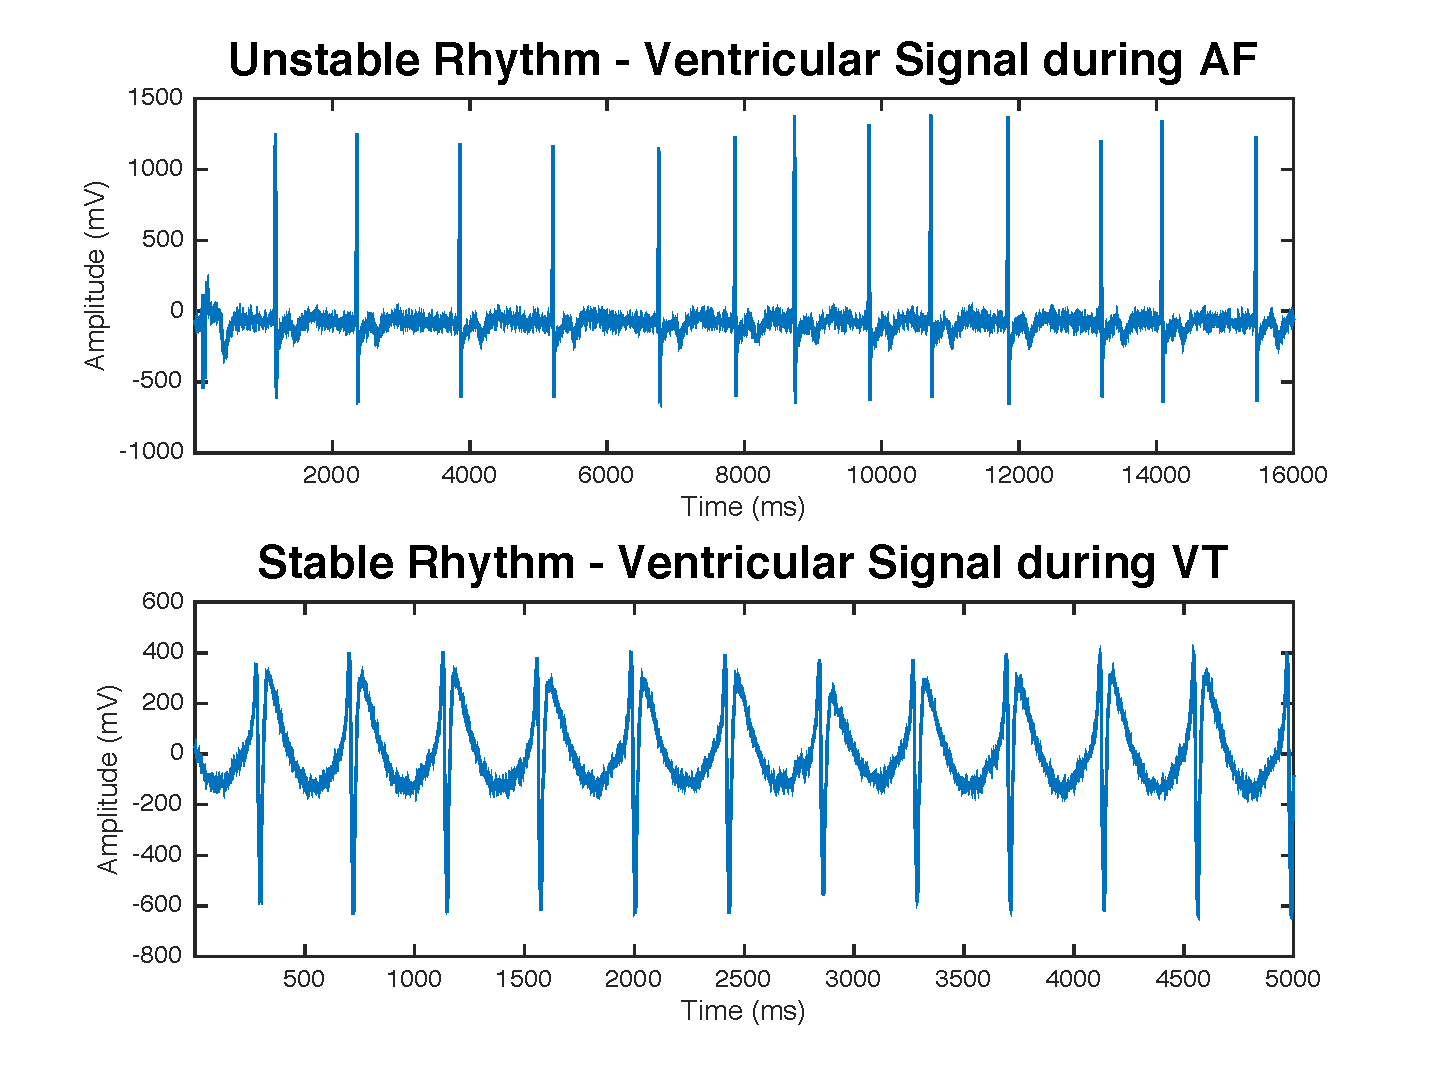
\includegraphics[scale=0.35]{figures/EGMStability}
%	\caption{Examples of a unstable rhythm (top) and stable rhythm (bottom).}
%	\label{fig:stable unstable}
%\end{figure}
\emph{Stability} refers to the variability of the peak-to-peak cycle length.
A rhythm with large variability (above a pre-defined threshold) is said to be \emph{unstable}, and is called stable otherwise.
The Stability discriminator is used to distinguish between atrial fibrillation, which is usually unstable, and \ac{VT}, which is usually stable.
%Atrial fibrillation, which is usually unstable, might induce a high ventricular rate .
%A \ac{VT}, on the other hand, is usually stable.
%Therefore this is a useful discriminator.

The Stability discriminator shown in Fig. \ref{fig:Hstab} simply calculates the variance of the cycle length over a fixed period called a Duration (measured in seconds).
Let $DL \geq 0$ be the Duration length.
\yhl{The events $DurationBegins?$ and $DurationEnds?$ indicate the transitions} of a simple system that measures the lapse of one Duration (not shown here).
State $t$ is a clock, $L_1$ accumulates the sum of interval lengths (and will be used to compute the average length), 
$L_2$ accumulates the squares of interval lengths,
and $\kappa$ is a counter that counts the number of accumulated beats.
$\sigma_2$ is assigned the value of the variance given by $\frac{1}{\kappa}[L_2 - L_1^2/\kappa]$
\begin{figure}[t]
	\centering
	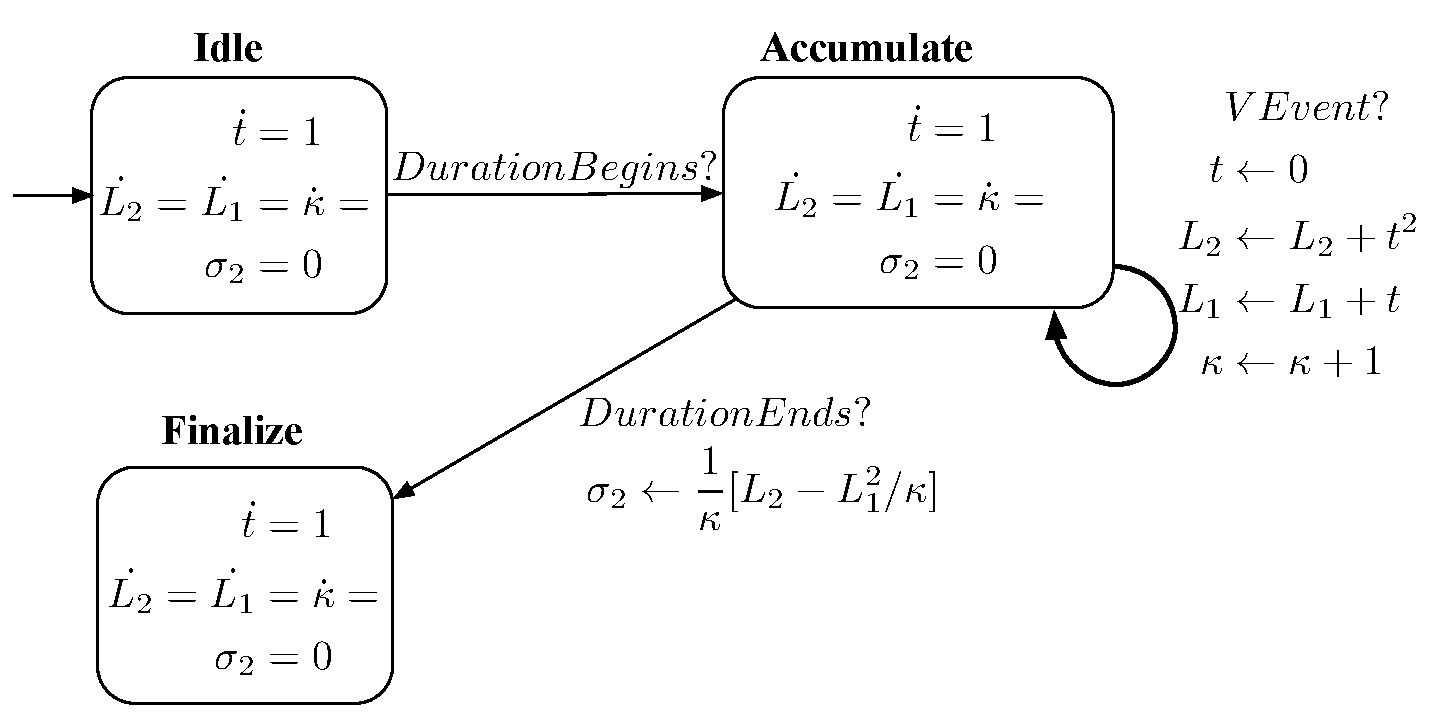
\includegraphics[scale=0.3]{figures/stability1v2}
	\vspace{-10pt}
	\caption{Stability discriminator.}
	\vspace{-10pt}
	\label{fig:Hstab}
\end{figure}

\begin{lemma}
	\label{lemma:stability}
	$\Sys_{Stab}$ is STORMED.	
\end{lemma}
The proof is in the Appendix.

Now that each system was shown to be STORMED, it remains to establish that their parallel composition is STORMED.
This result does not hold in general - Thm.~\ref{thm:SHS composition} gives conditions under which parallel composition respects the STORMED property.
Intuitively, we require that whenever a sub-collection of the systems jumps, the remaining systems that did not jump are separated from all of their respective guards by a uniform distance.
This is a requirement that can be shown to hold for our systems by modeling various minimal delays in the systems' operation. 
%For example, when a $VEvent?$ is issued by $\Sys_{Sense}$, $\Sys_{VTC}$ does not jump and will wait at least until the sampling time of the next fiducial point to make a transition.
%Or, when an atrial cell fires (in $\Sys_{CA}$), we model a minimal delay between it and all other cells that do not fire simultaneously.
We may now state:
\begin{thm}
Consider the collection of systems $\Sys_{CA}$, $\Sys_{ICD} = \Sys_{Sense} || \Sys_{Detection-Algo}$ where the latter is the parallel composition of the discriminator systems.
This collection satisfies the hypotheses of Thm. \ref{thm:SHS composition} (Section \ref{sec:compositionality}) and therefore the parallel system  $\Sys_{CA} || \Sys_{ICD}$ is STORMED and has a finite bisimulation.
\end{thm}